\section{Téléchargement des cours de la bourse}

Dans le cadre de ce projet nous avons besoin de 

\subsection{Yahoo! Finance}

\subsubsection{Présentation}

Yahoo! Finance est un site internet du groupe Yahoo! qui délivre des nombreuses informations dans le domaine de la finance. Ainsi, nous retrouvons une section actualité qui nous permet d'avoir un rapide coup d’œil sur les divers articles de journaux en rapport avec l'économie. Dans la partie vidéo le principe est le même sauf que les actualités sont sous forme de vidéos. \\

Yahoo propose de visualiser de nombreuses informations en rapport avec les cours ou indices. \\

Par exemple, pour l'indice du cac 40 n retrouve sa valeur ainsi que va variation par rapport à la dernière session. On a accès à la dernière valeur de clôture ainsi que la valeur à l'ouverture. Un graphique représente l'évolution du prix de l'indice depuis l'ouverture de la session. Nous avons également accès aux articles concernant le CAC40 dans la presse écrite, aux composants du CAC40 ainsi qu'aux prix historiques (valeur ouverture, fermeture, haut, bas sur la période désirée). \\


Pour un indice, ACCOR S.A dans notre exemple la page se présente comme suit : \\
\begin{figure}[!h]
  \center
  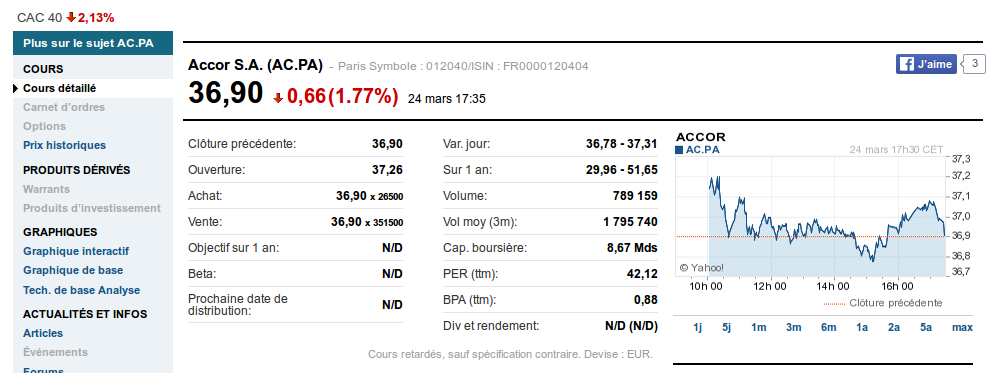
\includegraphics[scale=0.4]{../graph/yahoo.png} \\
  \caption{Visualisation du site Yahoo! Finance}
\end{figure}
Nous retrouvons les prix historiques (ce qui nous intéresse) ainsi que d'autres informations concernant le cours. 

